\chapter{The influence of the group environment}


\section{Group Identification}\label{sec:groups}

We used the \citet{berlind06} catalogue, which uses a friends-of-friends algorithm to identify group and cluster galaxies in the SDSS. This was cross matched to the \textsc{gz-galex} sample and limited to $z < 0.1$ to ensure GALEX completeness of the red sequence (see \citealt{ref}). Centrals were selected as the brightest galaxy in a group and all others were designated as satellites. This resulted in a sample of $14,199$ group galaxies with $3,468$ centrals and $10,731$ satellites within a projected cluster centric radius range of $0 < R/R_{200} < 25$ and $z < 0.084$. 

In this work we focus on galaxies which are either quenching or quenched and are more than $\pm1\sigma$ below the star forming `main sequence'. This encompasses $4629$ satellite and $2314$ central galaxies and will be referred to as the \textsc{gz-group} sample. {\notebsm These galaxies are highlighted in red on Figure \ref{}. }

\subsection{Field sample}\label{sec:field}

For all galaxies in the \textsc{gz-galex} sample, we calculated the smallest projected cluster centric radii from each of the central galaxies in the  \citet{berlind06} catalog and selected candidate field galaxies as those with (i) $R/R_{200} > 25$ and (ii) $\log\Sigma < -0.8$ from \cite{baldry06}. This sample of field galaxy candidates was then matched in redshift and stellar mass firstly to the central galaxies of the \textsc{gz-group} sample to give $2,309$ field galaxies with $z < 0.084$ which will be referred to as the \textsc{gz-cent-field} sample. Secondly, the field galaxy candidates were then matched in redshift and stellar mass to the satellite galaxies of the \textsc{gz-group} sample to give $6,849$ field galaxies with $z < 0.084$ which will be referred to as the \textsc{gz-sat-field}. These galaxies in the \textsc{gz-sat-field} sample will be used as a control when investigating the morphological trends of satellite galaxies with environment. 

As in Section \ref{sec:groups} we select all those galaxies in the central matched sample $\pm1\sigma$ below the star forming `main sequence', giving $1596$ quenching or quenched field galaxies for use as a control sample, which will be referred to as the \textsc{gz-cent-field-q} sample. These galaxies will be used as a control when investigating the quenching parameters of the different environments in order to ensure that each galaxy under comparison resides in similar stellar mass halos. 
%We also select all those galaxies in the satellite matched sample $\pm1\sigma$ below the star forming `main sequence', giving $$ quenching or quenched field galaxies for use as a control sample, which will be referred to as the \textsc{gz-sat-field-q} sample.
  
\begin{figure*}
\centering{
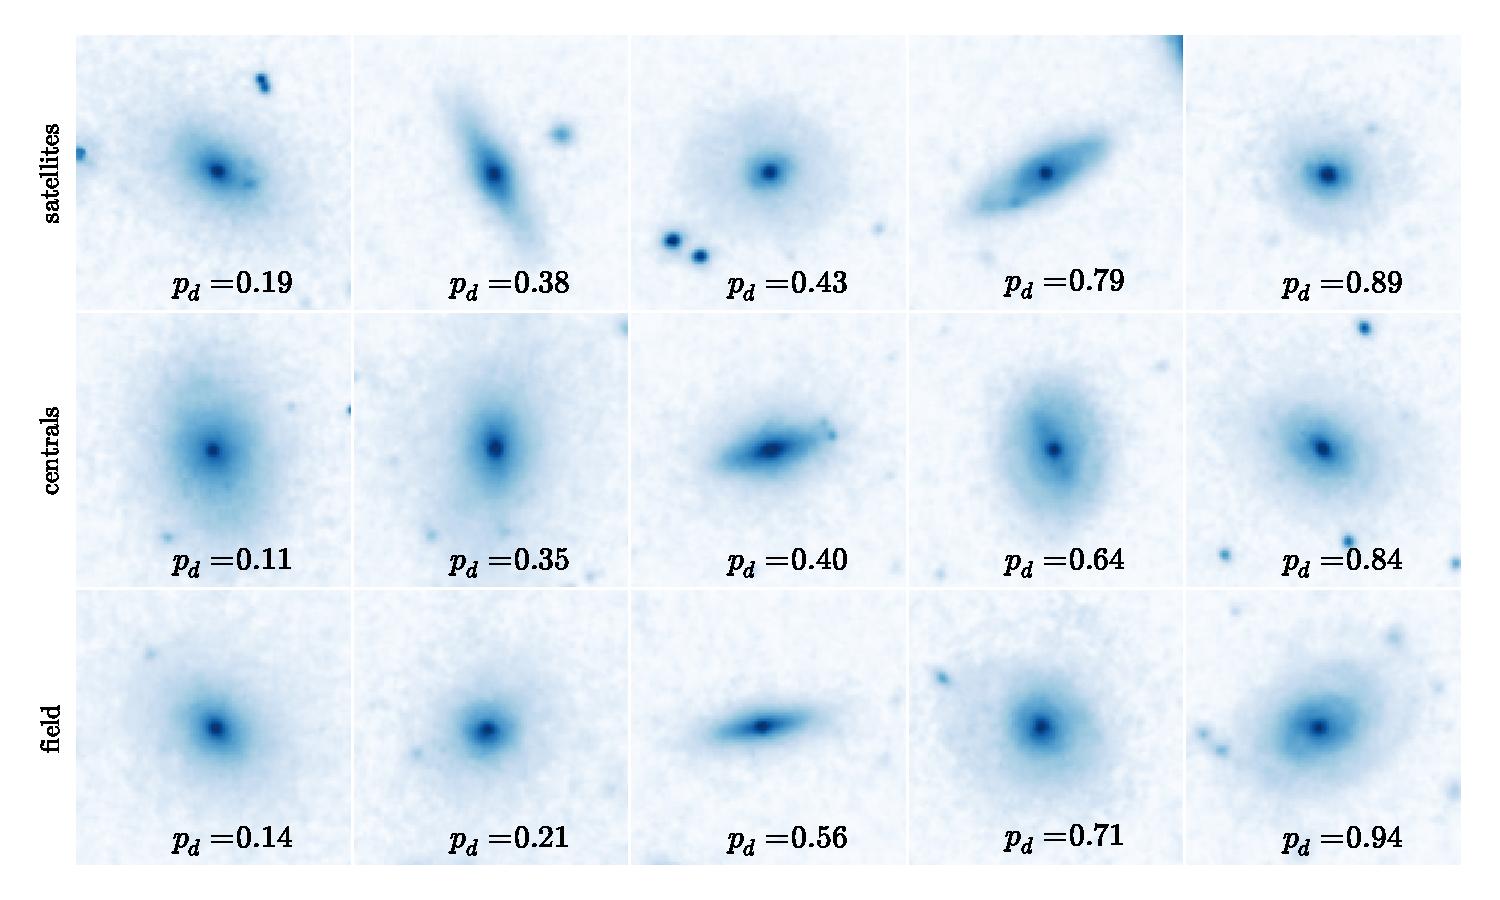
\includegraphics[width=0.95\textwidth]{environment/mosaic_sat_cent_field_disc_fraction.pdf}
\caption[SDSS images of galaxies in the \textsc{gz-group} and  \textsc{gz-field} samples]{Randomly selected SDSS \emph{gri} composite images of satellite and central galaxies in the \textsc{gz-group} sample in comparison to those from the \textsc{gz-field} sample. All galaxies lie within $0.04 < z < 0.05$ and in the central galaxy mass range $10^{10.5} < M_{*} [M_{\odot}] < 10^{11}$, used as a proxy for halo mass. The galaxies are ordered from least to most featured according to their debiased `disc or featured' vote fraction, $p_d$ (see \citealt{GZ2}). The scale for each image is $0.099~\rm{arcsec/pixel}$.}}
\label{fig:mosaic}
\end{figure*}

\begin{figure}
\centering{
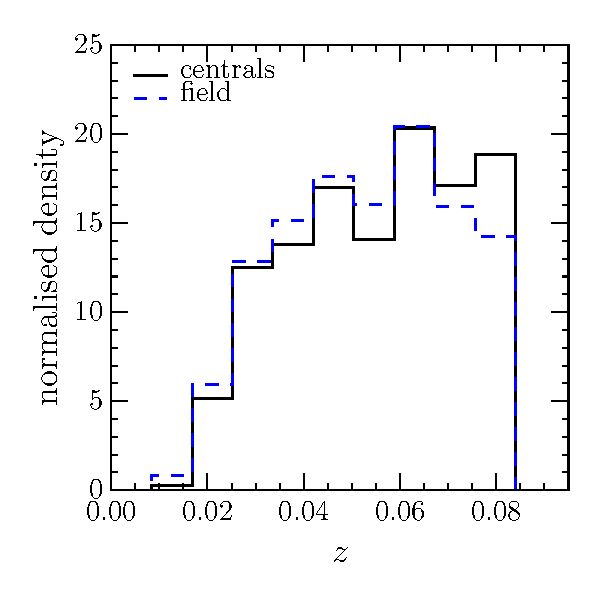
\includegraphics[width=0.8\textwidth]{environment/redshift_cent_field.pdf}
\caption[Redshift distribution comparison of the \textsc{gz-group} sample and matched control \textsc{gz-cent-field-q} sample]{Redshift distributions of quenching or quenched central galaxies in the \textsc{gz-group} sample (black solid line) in comparison to the redshift and mass matched \textsc{gz-cent-field-q} sample (blue dashed line).}}
\label{fig:zcompare}
\end{figure}

\section{Results}\label{sec:results}

\begin{figure}
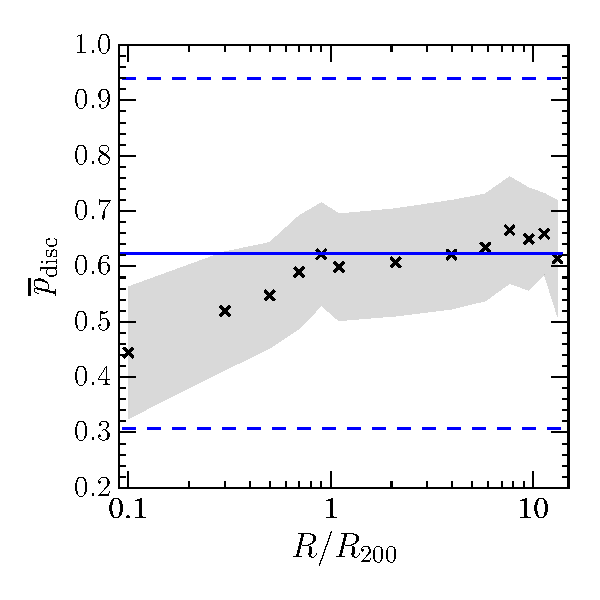
\includegraphics[width=0.46\textwidth]{environment/p_disc_trend_with_log_radius_field_compare.pdf}
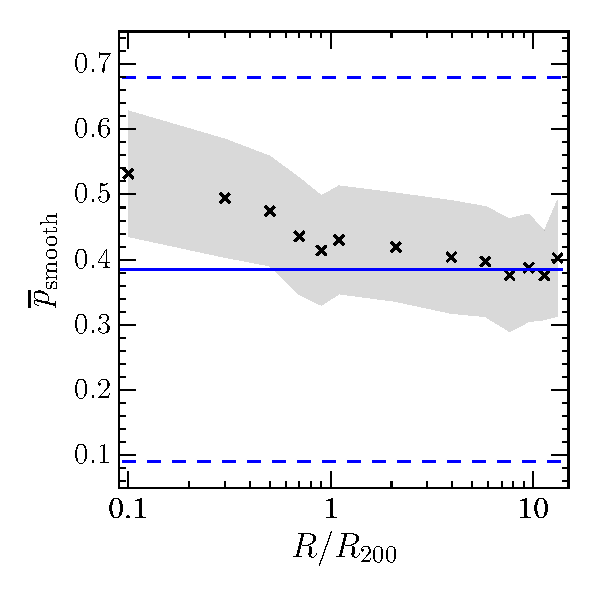
\includegraphics[width=0.46\textwidth]{environment/p_smooth_trend_with_log_radius_field_compare.pdf}
\caption[Mean GZ vote fractions for satellite galaxies with projected cluster centric radius]{Mean GZ vote fraction for disc (top) and smooth (bottom) galaxies in the \textsc{gz-group} sample binned in projected cluster centric radius, normalised by $R_{200}$, a proxy for the virial radius of a group. The shaded region shows $\pm1\sigma$ on the mean vote fraction. The mean vote fraction of the \textsc{field} sample are also shown (blue solid lines) with $\pm1\sigma$ (blue dashed lines).}
\label{fig:morphradius}
\end{figure}

\begin{figure}
\centering{
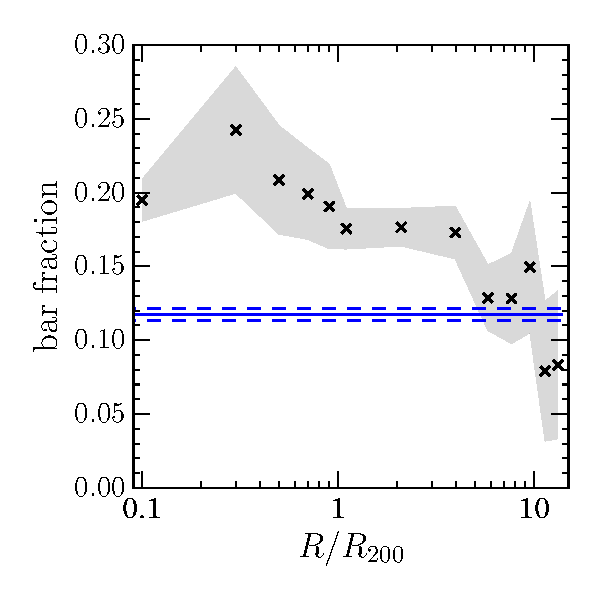
\includegraphics[width=0.95\textwidth]{environment/bar_fraction_over_disc_trend_with_log_radius_sat_matched_field_cand.pdf}
\caption[Bar fraction of satellite disc galaxies with projected cluster centric radius]{Bar fraction (number of barred disc galaxies over number of disc galaxies) in the \textsc{gz-group} sample binned in projected cluster centric radius, normalised by $R_{200}$, a proxy for the virial radius of a group. The shaded region shows $\pm1\sigma$ on the bar fraction. The bar fraction of the \textsc{gz-sat-field} sample is also shown (blue solid line) with $\pm1\sigma$ (blue dashed line).}}
\label{fig:barradius}
\end{figure}

\begin{figure}
\centering{
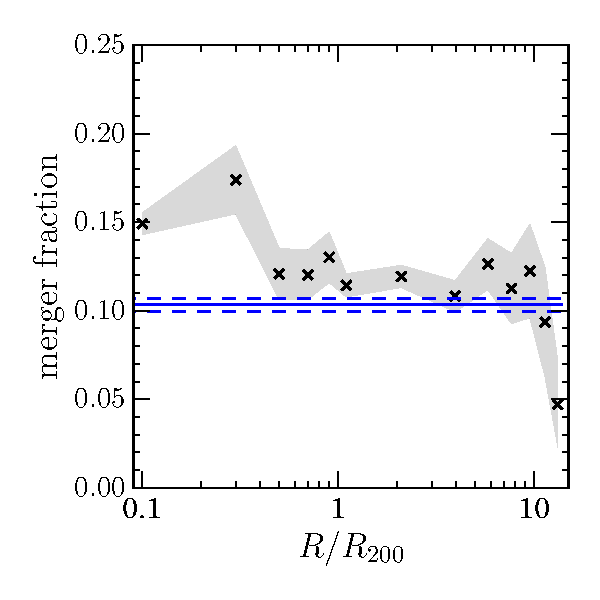
\includegraphics[width=0.95\textwidth]{environment/merger_fraction_trend_with_log_radius_compare_sat_field_cand.pdf}
\caption[Merger fraction of satellite galaxies with projected cluster centric radius]{Merger fraction in the \textsc{gz-group} sample binned in projected cluster centric radius, normalised by $R_{200}$, a proxy for the virial radius of a group. The shaded region shows $\pm1\sigma$ on the merger fraction. The merger fraction of the \textsc{gz-sat-field} sample is also shown (blue solid line) with $\pm1\sigma$ (blue dashed line).}}
\label{fig:mergerradius}
\end{figure}

\begin{figure*}
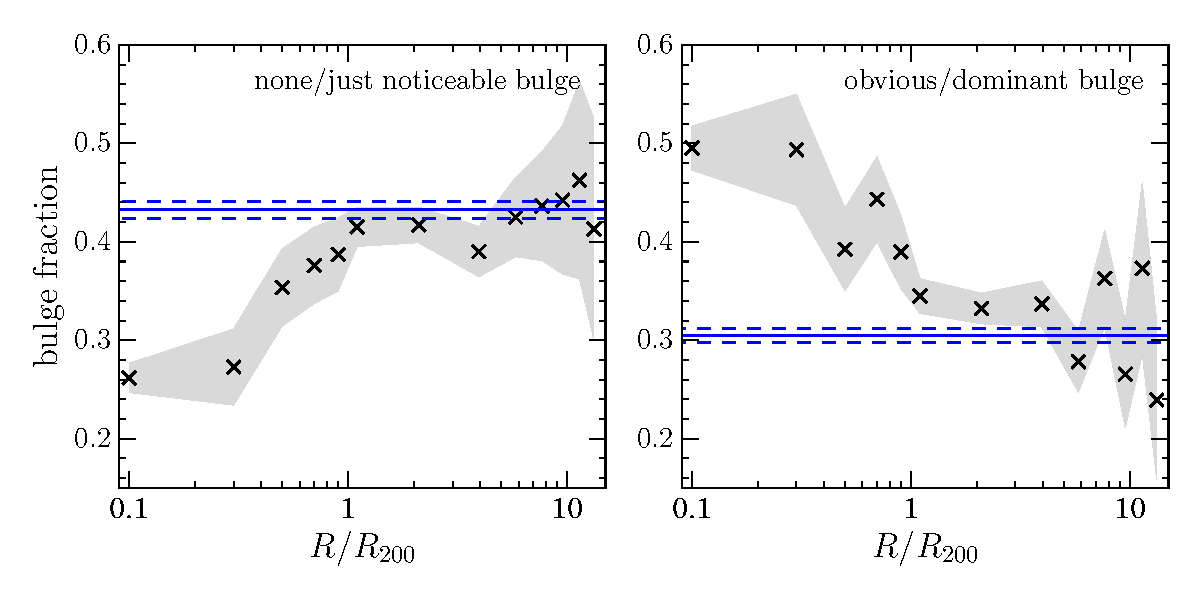
\includegraphics[width=\textwidth]{environment/min_max_bulge_fraction_trend_with_log_radius_sat_field_cand.pdf}
\caption[GZ2 bulge fractions of satellite disc galaxies with projected cluster centric radius]{Fraction of galaxies with none/just noticeable bulge classifications (left) and with obvious/dominant bulge classifications (right) in the \textsc{gz-group} sample binned in projected cluster centric radius, normalised by $R_{200}$, a proxy for the virial radius of a group. The shaded regions shows $\pm1\sigma$ on the bulge fractions. The bulge fractions of the \textsc{gz-sat-field} sample are also shown (blue solid lines) with $\pm1\sigma$ (blue dashed lines).}
\label{fig:bulgeradius}
\end{figure*}

\begin{figure}
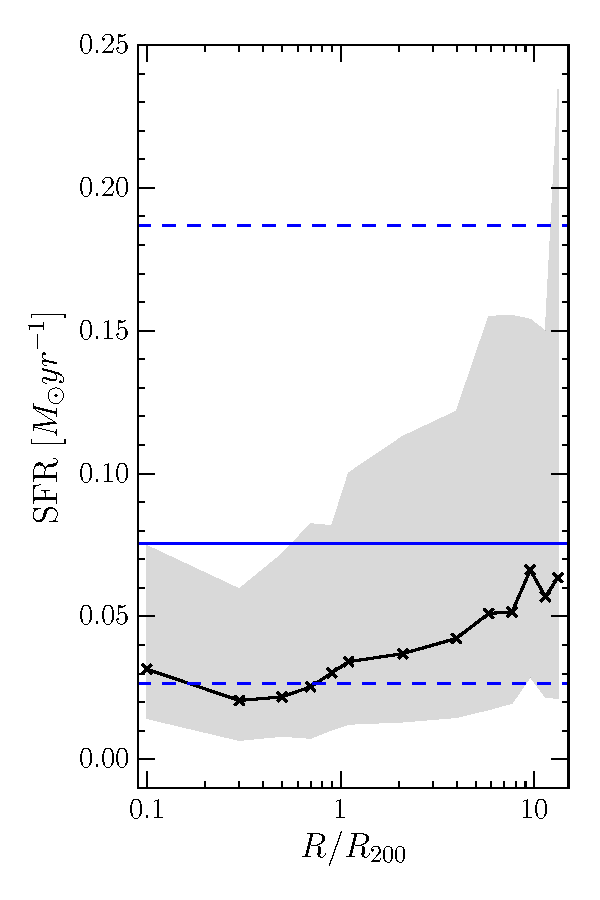
\includegraphics[height=0.825\textheight]{environment/sfr_trend_with_log_radius_field_matched_blue_dashed_hlines_gomez_03_rv_not_r200.pdf}
\caption[Median SFR of the \textsc{gz-group} sample with projected cluster centric radius]{Median $H\alpha$ derived star formation rates of satellite galaxies in the \textsc{gz-group} sample, binned in projected cluster centric radius, normalised by $R_{200}$, a proxy for the virial radius of a group.  The shaded region shows the SFRs encompassed by $50\%$ of the population in a given bin. The median SFR of the \textsc{gz-sat-field} sample is shown (blue solid line) along with the 25th and 75th percentiles (blue dashed lines).}
\label{fig:sfrradius}
\end{figure}


With the output from \starpy~ we can also study the time since quenching onset ($\Delta t = t_{obs} - t_{q}$, see Section \ref{}) binned in projected cluster centric radius, normalised by $R_{200}$ (a proxy for virial radius) for satellite galaxies and central galaxies in the \textsc{gz2-group} sample, compared with galaxies in the \textsc{gz2-field} sample. We can investigate these trends with group properties as shown in Figures \ref{fig:timesinceradius} \& \ref{fig:timesinceradiusvel}. 

Across all the panels in Figures \ref{fig:timesinceradius} \& \ref{fig:timesinceradiusvel} we see a general trend for increasing time since quenching onset with decreasing distance from the group centre, which is suggestive that this trend is due to an environmental quenching mechanism. As earlier, in Figures \ref{fig:morphradius}$-$\ref{fig:bulgeradius} significant differences from the field value arise inside $\sim$ one virial radius. 

If mergers are an important evolutionary mechanism for satellite galaxies as the morphological evidence in Figures~\ref{fig:mergerradius} \& \ref{fig:bulgeradius} suggests, we would expect to see a difference in the quenching histories of satellites in groups with a higher number of galaxies, $N_{group}$. However, the bottom panel of Figure \ref{fig:timesinceradius} shows that there is no trend with time since quenching onset with increasing $N_{group}$ for the satellite galaxies. The central galaxies (shown by the square points at $\sim 0.01 R/R_{200}$) however, do show a trend for increasing time since quenching with $N_group$. Suggesting that mergers are not the dominant quenching mechanism for satellite galaxies but are for centrals.  

In the middle panel of Figure \ref{fig:timesinceradius} the satellite galaxies of the \textsc{gz2-group} sample are now split by their stellar mass (calculated from the absolute r-band magnitude and $u-r$ colour by the method outlined in \citealt{baldry06}) and we do see a clear trend for increasing time since quenching onset with increasing stellar mass for both satellite and central galaxies. This is suggestive of mass quenching among the group galaxy population. This is contrary to previous work suggesting that mass quenching is only of import for central galaxies \citep{ref, ref, ref}. Interestingly, the inner satellites of a given mass have quenched less recently than the centrals at the same mass range, suggesting some episode of more recent star formation may have occurred in the central galaxies but not in the inner satellites. This is once again suggestive of a merger dominated evolutionary history for central galaxies, with mergers postulated to cause a burst of star formation before then quenching the remnant galaxy \citep{?,?, pontzen16}. 

In simulations, the three things that are found to most constrain galaxy evolution are redshift, mass and halo mass \cite{ref, ref}. To study the effect that halo mass has on the quenching properties of group galaxies we shall use a proxy for halo mass by splitting by the \textsc{gz2-group} sample by the stellar mass of the corresponding central galaxy of a group.

This is shown in the top panel of Figure \ref{fig:timesinceradius} where we can once again see a clear trend for increasing time since quenching onset with increasing stellar mass of the group central for both satellite and central galaxies. More massive halos therefore have a greater impact on the star formation histories of their satellites than less massive halos. This is often though to be attributed to hotter inter galactic medium (IGM) temperatures in higher mass halos which can then impact on a galaxy through ram pressure stripping (RPS) of gas for star formation. If RPS is indeed a dominant environmental quenching mechanism we should therefore see a trend in $\Delta t$ with the speed of a satellite galaxy relative to the group central.  In the bottom panel of Figure \ref{fig:timesinceradiusvel} we split the satellite galaxies of the \textsc{gz2-group} sample into bins of relative velocity to their central galaxies. We can see that there is no trend with time since onset of quenching with increasing relative velocity for satellite galaxies, however the trend with decreasing projected group centric radius, seen in each panel in Figure \ref{fig:timesinceradius} is still present. This suggests that any environmental processes causing this quenching are not corrected with satellite velocity and therefore RPS is not the dominant environmental quenching mechanism, in support of the conclusions of \citep{?}.

We can also account for both the stellar mass and the halo mass of the central galaxy simultaneously by considering the stellar mass ratio of the satellite to it's central galaxy, $\mu_* = M_*/M_{*,c}$, once again using the stellar mass of the central galaxy as a proxy for halo mass. In the middle panel of Figure \ref{fig:timesinceradiusvel} we show the time since quenching of the \textsc{gz2-group} sample with projected cluster centric radius split into bins of $\mu_*$. The change in $\Delta t $ with projected cluster centric radius occurs more steeply (particularly beyond $\sim$ a virial radius) for satellite galaxies with much smaller masses than their group central ($-2.0 < \log_{10}\mu_* < -1.0$, shown by the blue curve). Since the stellar mass of the central galaxy is correlated with the halo mass and therefore the potential of the system, this suggests that smaller mass galaxies in larger halos are most effected by environmental effects, therefore the dominant environmental quenching mechanism must be correlated with the group potential. 

Previous studies have claimed that the property which correlates most with whether a galaxy is quenched is the stellar velocity dispersion, $\sigma_*$. Shown in the top panel of Figure \ref{fig:timesinceradiusvel} is the time since quenching of the \textsc{gz2-group} sample with projected cluster centric radius split into bins of $\sigma_*$. Along with the stellar mass (shown in the middle panel of Figure \ref{fig:timesinceradius}), the stellar velocity dispersion shows the largest trend in $\Delta t$  for satellite galaxies, with galaxies with the smallest (largest) stellar velocity dispersions have quenched more (less) recently. 

\begin{figure}
\centering{
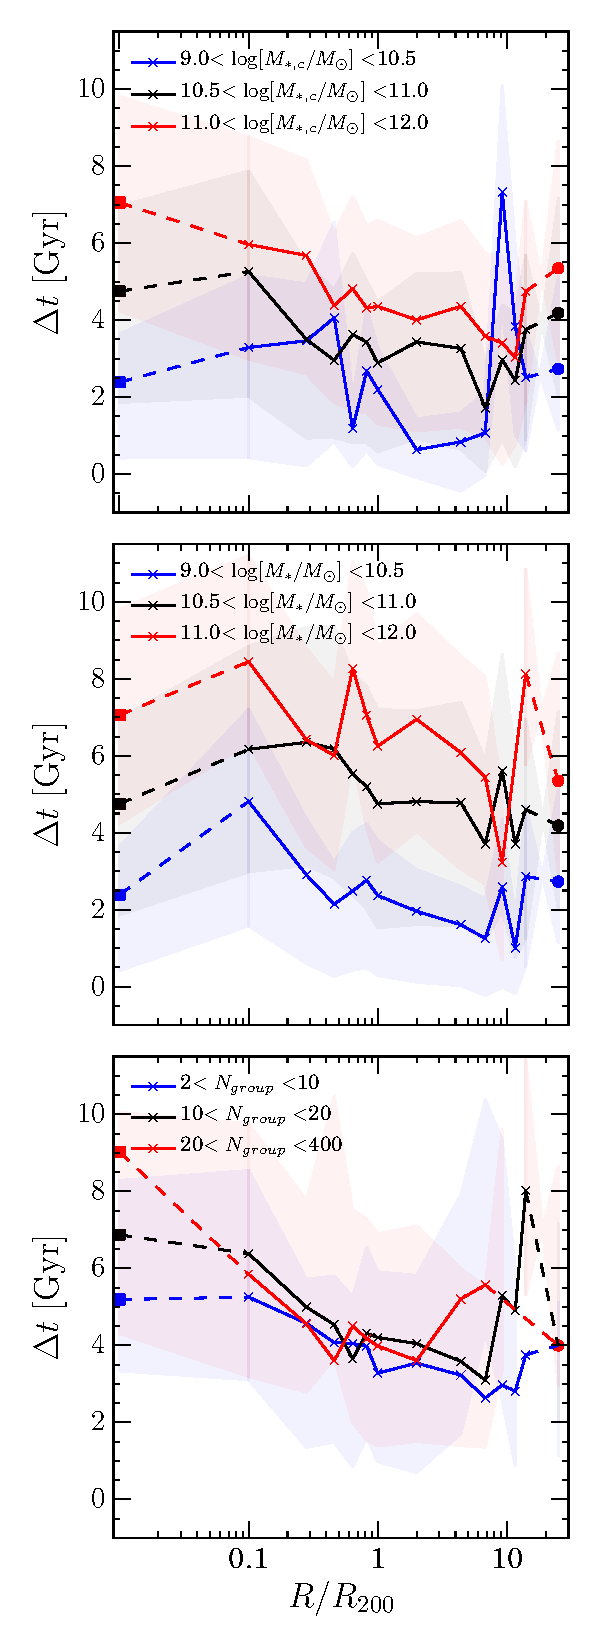
\includegraphics[height=0.825\textheight]{environment/time_since_quenching_environment_properties.pdf}
\caption[The time since quenching of the \textsc{gz-group} sample with projected cluster centric radius]{The time since quenching onset ($\Delta t = t_{obs} - t_{q}$) binned in projected cluster centric radius, normalised by $R_{200}$, for satellite galaxies (triangles) split by stellar mass of the corresponding central galaxy (top), stellar mass (middle) and the number of galaxies within the group (bottom). The corresponding values for central galaxies (squares) and galaxies in the \textsc{gz-cent-field} sample (circles) are shown and connected by the dashed lines to aid the reader.}
\label{fig:timesinceradius}}
\end{figure}

\begin{figure}
\centering{
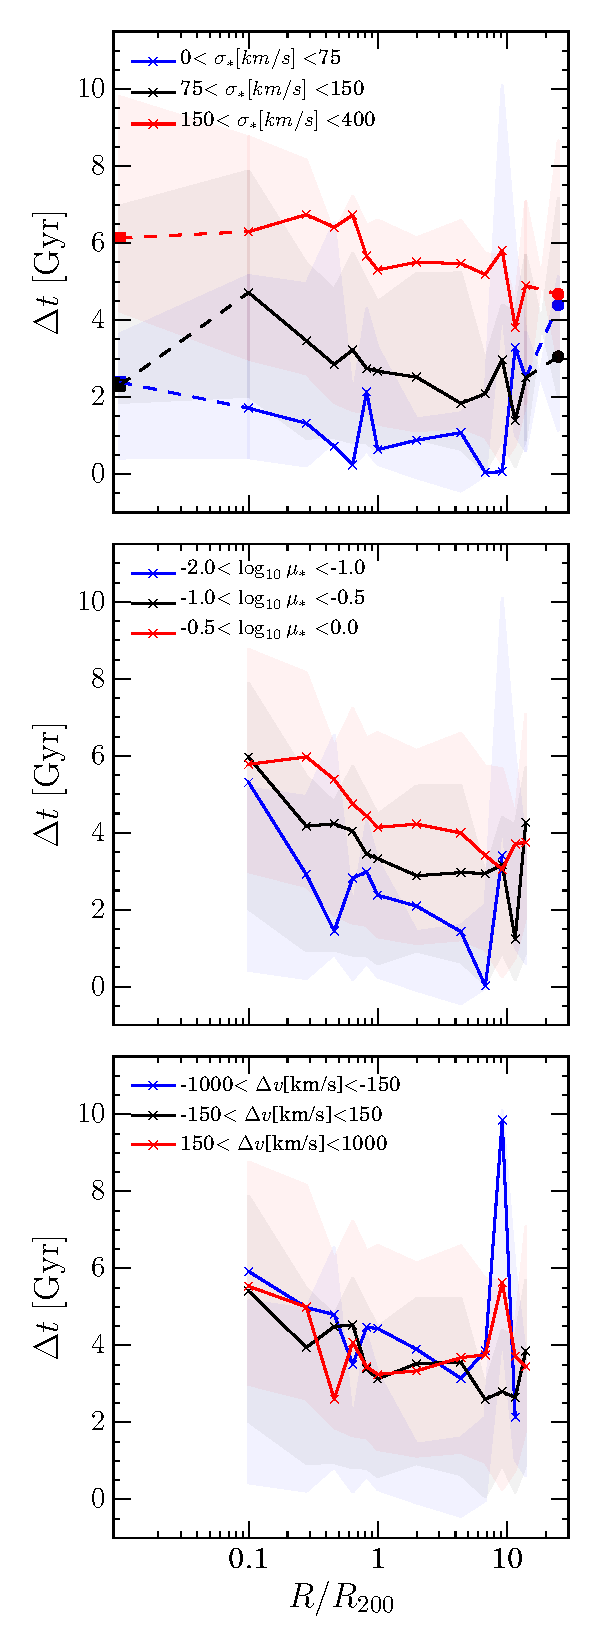
\includegraphics[height=0.825\textheight]{environment/time_since_quenching_v_disp_mu_bins_delv.pdf}
\caption[The time since quenching of the \textsc{gz-group} sample with projected cluster centric radius]{The time since quenching onset ($\Delta t = t_{obs} - t_{q}$) binned in projected cluster centric radius, normalised by $R_{200}$, for satellite galaxies (triangles) split by velocity dispersion (top), stellar mass ratio ($\mu_* = M_*/M_{*,c}$) (middle) and the difference in velocity from the associated central galaxy (bottom). The corresponding values for central galaxies (squares) and galaxies in the \textsc{gz-cent-field} sample (circles) are shown and connected by the dashed lines to aid the reader in the top panel where appropriate.}
\label{fig:timesinceradiusvel}}
\end{figure}


\section{Discussion}\label{sec:disc}

Across all panels of Figures ~\ref{fig:timesinceradius}-\ref{fig:timesinceradiusvel} a trend for increasing time since quenching onset with decreasing projected cluster centric radius was present. This suggests that the environment does directly cause quenching; galaxies closer in, fell into the group earlier and as they did so they started to quench giving rise to a larger $\Delta t$. However, as seen in Figure \ref{fig:timesinceradiusvel} there is no trend in the time since quenching onset with the relative velocity of the satellites to their corresponding central and a steeper trend with $R/R_{200}$ for lower mass satellites in larger mass halos. This suggests that whatever environmental mechanism is at play here, it is dependant on the size of the halo, either due to the potential or temperature of the halo, but not dependant on the speed of the satellite. This suggests that ram pressure stripping is not the dominant environmental quenching mechanism at play. 

We have shown that mergers are important for centrals not for satellites in the bottom panel of Figure \ref{fig:timesinceradius}. That mass quenching is important for satellites as well as centrals in the middle panel of Figure \ref{fig:timesinceradius} and that larger halos have a stronger environmental effect on their satellites in the top panel of Figure \ref{fig:timesinceradius}. 

